\subsection{Robot Design}\label{subsec:robot-design}
For this project, we elected to use a flying Tello drone.
We chose a flying drone primarily because it can easily bring its camera into detection range of apples in a tree, regardless of height.
A flying drone also has the advantage of not disturbing or caring about the terrain, which may be muddy or bumpy in some orchards.

However, flying drones suffer from a number of disadvantages.
The two primary difficulties are the lack of computational power and the lack of battery life.
A typical drone is unable to remain in the air long enough to both approach apples and determine their ripeness, and are  additionally too slow to use some of the heavier models in a reasonable time-frame.
As such, in order to overcome these challenges we developed an intelligence hierarchy to only perform calculations as required, and offloaded these calculations to an external ``controller'' computer.

The intelligence hierarchy is outlined in \autoref{fig:intelligence-hierarchy}.
The controller starts by detecting if an apple if is in view, then proceeds to calculate its position relative to the apple and approach it.
Finally, models are used to detect the ripeness of the apple, as well as if it is rotten.

The data flow for the hierarchy can be seen in \autoref{fig:fruit-fly-model-diagram}.
Each step occurs sequentially, and the next one only occurs when the previous one completes successfully.
For example, the drone will not calculate its position relative to an apple if it does not detect an apple, nor will it detect its ripeness.
This setup removes the burden from the drone, while also minimizing the calculations done by the controller.

\begin{figure}[!htb]
    \fontsize{7}{5}\selectfont
    \centering
    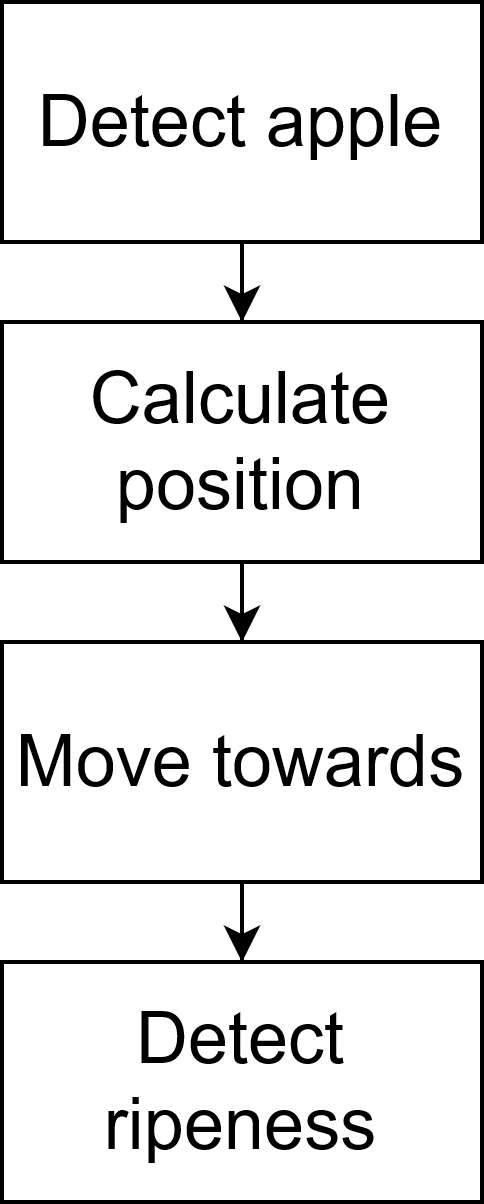
\includegraphics[scale=0.8]
    {./figures/intelligence-hierarchy}
    \caption{
        The intelligence hierarchy used by the drone.
        Each layer is designed to minimize the work done by the controller so it does not perform expensive calculations except when needed.
    }
    \label{fig:intelligence-hierarchy}
\end{figure}

\begin{figure}[!htb]
    \fontsize{7}{5}\selectfont
    \centering
    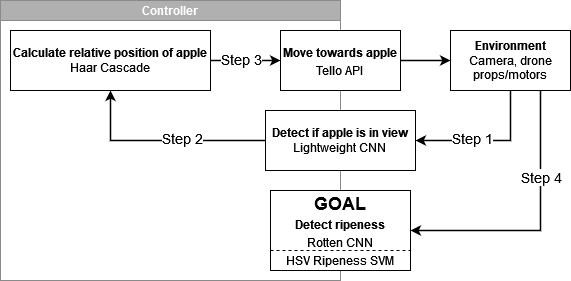
\includegraphics[width=\columnwidth,keepaspectratio]
    {./figures/fruit-fly-model-diagram}
    \caption{
        A data flow diagram of how the intelligence hierarchy works.
        The controller, which operates on another machine receives input from the drone's cameras and other sensors.
        This information is passed to a lightweight model, then to heavier models to operate the drone and determine fruit ripeness.
    }
    \label{fig:fruit-fly-model-diagram}
\end{figure}
